% -------------------
% CONTEXTE HISTORIQUE
% -------------------

% Defining TOC's sections before content
\section*{Un peu d'histoire}

\begin{frame}{Un peu d'histoire}
    \begin{columns}
        \column{0.55\linewidth}
        Déçu de la qualité d'impression de son livre \textit{The Art of Computer Programming},
        il créa \TeX\;en 1977.
        \vspace{0.5cm}
        \begin{itemize}
            \item[$\diamond$] Simplicité, reproductibilité et pérennité
            \item[$\diamond$] Gestion des polices et caractères mathématiques
        \end{itemize}
        \column{0.5\linewidth}
        \begin{figure}
           \centering
            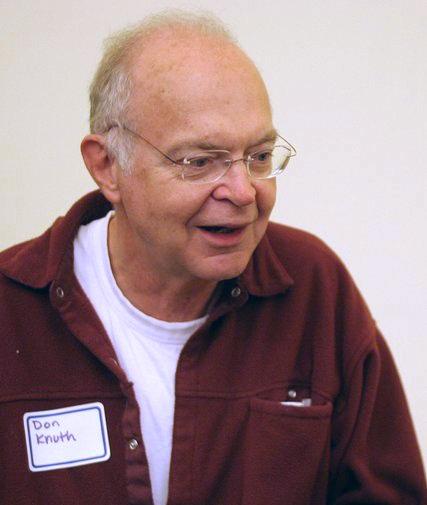
\includegraphics[scale=0.35]{./figures/KnuthAtOpenContentAlliance.jpg}
            \caption{\cite{DON}}
            \label{fig: DONALD}
        \end{figure}
    \end{columns}
\end{frame}

\begin{frame}{Un peu d'histoire}
    \begin{columns}
        \column{0.5\linewidth}
        Trouvait \TeX\; trop laborieux pour les non-experts.
        Il créa \LaTeX\; en 1983.
        \vspace{0.5cm}
        \begin{itemize}
            \item[$\diamond$] Interface \textit{high-level} de\;\TeX
            \item[$\diamond$] Classe de document~: \textit{article}, \textit{book}, \textit{rapport}, etc.
            \item[$\diamond$] Devient modulaire et personnalisable grâce aux \textit{packages}
        \end{itemize}
        \column{0.5\linewidth}
        \begin{figure}
           \centering
            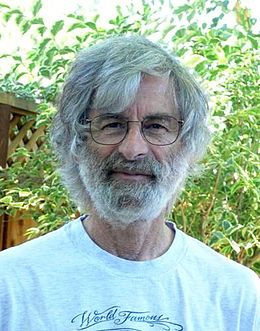
\includegraphics[scale=0.45]{./figures/Leslie_Lamport.jpg}
            \caption{\cite{LAMPORT}}
            \label{fig: LESLIE}
        \end{figure}
    \end{columns}
\end{frame}
